\documentclass{article}

\usepackage{mathtools,amsfonts}
\usepackage{enumerate}
\usepackage{fancyvrb}
\usepackage{graphicx}
% \usepackage{fullpage}
\graphicspath{ {./} }


\begin{document}
\thispagestyle{empty}

\begin{center}
  \textbf{\Large Junior Test 1}
  % LEVEL is Senior, Intermediate or Beginner
  % NUMBER is the test number: 1, 2, etc.
  \\ \vspace{1em}
  \textbf{\large Stellenbosch Camp 2019}
  \\ \vspace{1em}
  \textbf{\large Time: $2\frac{1}{2}$ hours}
\end{center}

\vspace{6.81mm}

\begin{enumerate}[1.]

\item % SAMO
a) The numbers $1$ through $12$ must be filled into the circles such that the sum along each line is $32$. Do it!

\begin{center}
    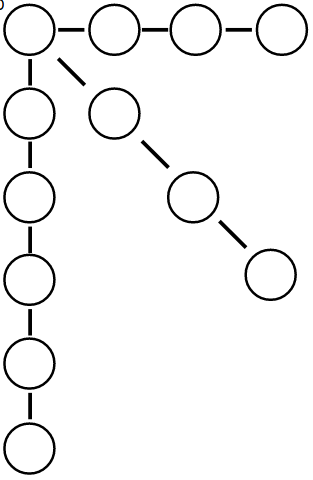
\includegraphics[width=0.2\textwidth]{test_1_question_1}
\end{center}
b) The numbers $1$ through $12$ are arranged in the circles such that each sum is $S$. What are the possible values of $S$?
\vspace{6.81mm}


\item % SAMO
~
\begin{center}
    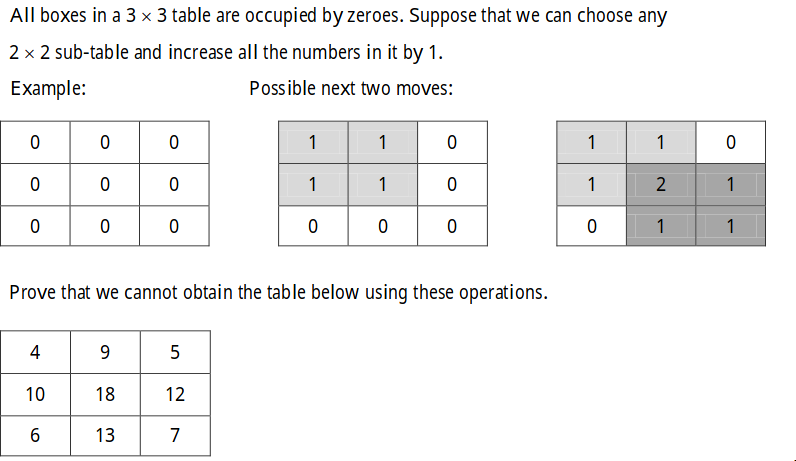
\includegraphics[width=0.9\textwidth]{test_1_question_2}
\end{center}
\vspace{6.81mm}


\item % SAMO
~
\begin{center}
    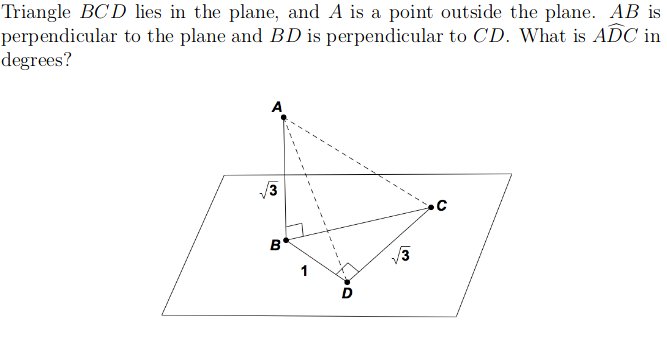
\includegraphics[width=0.9\textwidth]{test_1_question_3}
\end{center}
\vspace{6.81mm}


\item % Standard
You are a citizen of Amestris, living your life as an aspiring Mathematician, but ho! One day, you find yourself in a conundrum! You found a compass on sale, but you cannot make the exact value with the \$7 and \$11 that Amestris trades in. 

What is the maximal value of the compass?
\vspace{6.81mm}


\item % Venezuela Final Round 2019, Q4
If $x + \frac{1}{x} = 3$, what is the value of $x^5 + \frac{1}{x^5}$?

\end{enumerate}


\vfill
% ASCII art
\begin{center}
\begin{BVerbatim}
   .___,   
___('v')___
`"-\._./-"'
    ^ ^ 

\end{BVerbatim}
\end{center}

\end{document}
